\subsection{External interface requirements}
\subsubsection{User interfaces}
\begin{@empty}
The following mockups show an approximation of the mobile application.\\

\setlength{\intextsep}{10pt plus \textheight minus 10pt}

\begin{figure}[H]
\centering
\begin{minipage}{.4\textwidth}
    \centering
    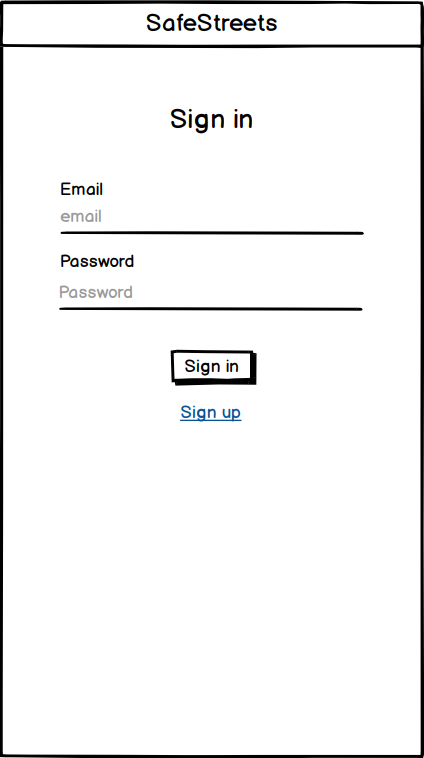
\includegraphics[width=.8\textwidth]{Images/sign-in.png}
    \caption{\label{fig:mockup-sign-in}Mockup - Sign in.}
\end{minipage}
\begin{minipage}{.4\textwidth}
    \centering
    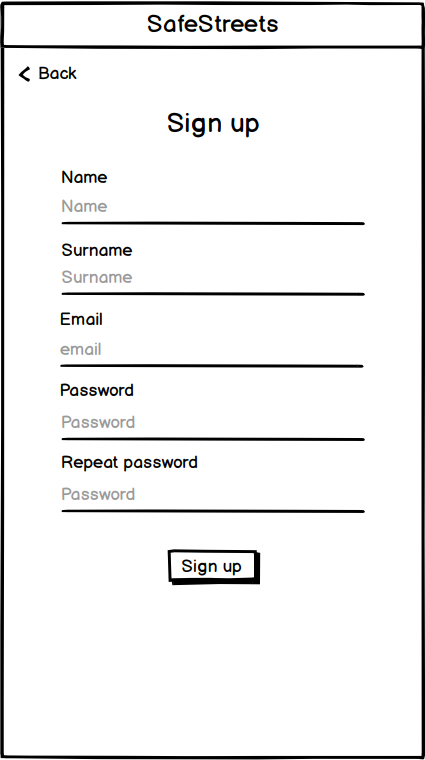
\includegraphics[width=.8\textwidth]{Images/sign-up.png}
    \caption{\label{fig:mockup-sign-up}Mockup - Sign up.}
\end{minipage}
\end{figure}

\begin{figure}[H]
\centering
\begin{minipage}{.4\textwidth}
    \centering
    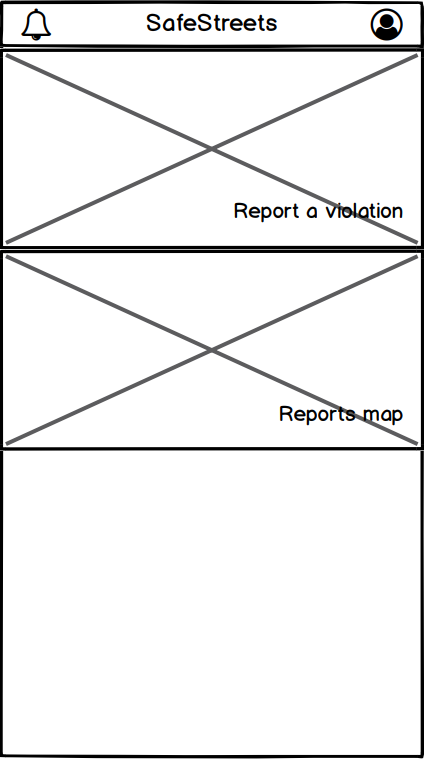
\includegraphics[width=.8\textwidth]{Images/home.png}
    \caption{\label{fig:mockup-home}Mockup - Home.}
\end{minipage}
\begin{minipage}{.4\textwidth}
    \centering
    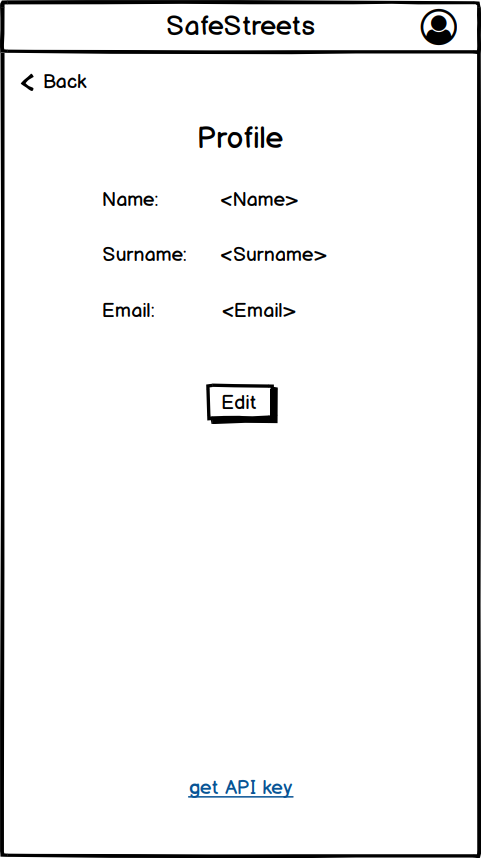
\includegraphics[width=.8\textwidth]{Images/profile.png}
    \caption{\label{fig:mockup-profile}Mockup - Profile.}
\end{minipage}
\end{figure}

\begin{figure}[H]
\centering
\begin{minipage}{.4\textwidth}
    \centering
    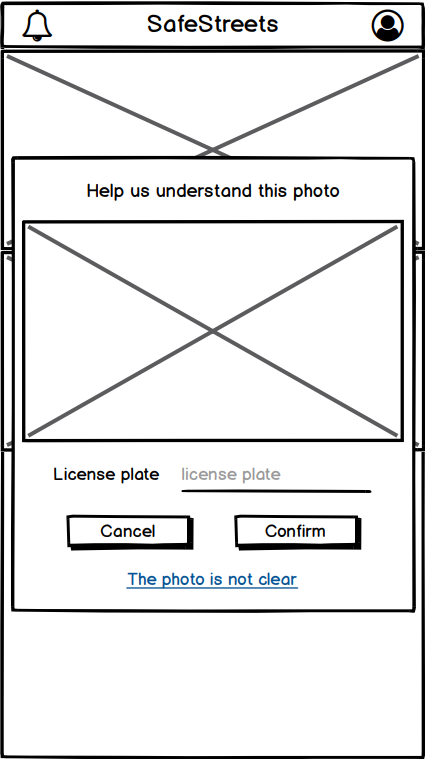
\includegraphics[width=.8\textwidth]{Images/photo-review.png}
    \caption{\label{fig:mockup-photo-review}Mockup - Photo review.}
\end{minipage}
\begin{minipage}{.4\textwidth}
    \centering
    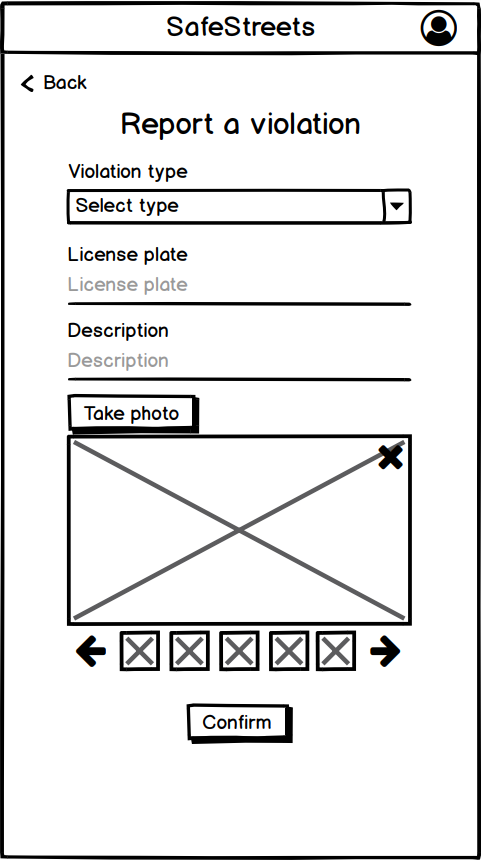
\includegraphics[width=.8\textwidth]{Images/report-violation.png}
    \caption{\label{fig:mockup-report-violation}Mockup - Report violation.}
\end{minipage}
\end{figure}

\begin{figure}[H]
\centering
\begin{minipage}{.4\textwidth}
    \centering
    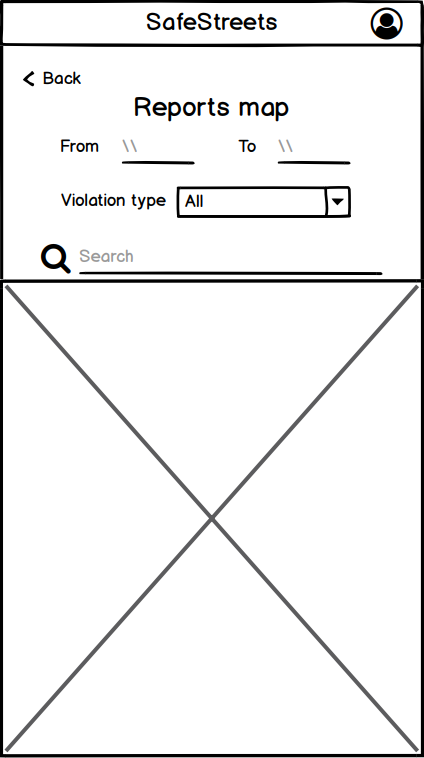
\includegraphics[width=.8\textwidth]{Images/reports-map.png}
    \caption{\label{fig:mockup-reports-map}Mockup - Reports map.}
\end{minipage}
\end{figure}
\end{@empty}

\subsubsection{Hardware interfaces}
\subsubsection{Software interfaces}
\begin{itemize}
\item
License plate recognition: An external library or API is necessary to perform license plate recognition on the photos submitted and determine the validity of a report.
\item
Car recognition: To determine the legitimacy of a report, a way to detect cars in the photos is essential. Thanks to this, it can be ensured that the license plate is attached to a car. Also, by cross referencing the characteristics of the car with the license plate registry, it can be ensured that there was no swapping of license plates.
\item
License plate registry: Access to the local government’s license plate registry is needed to be able to cross reference the detected license plate and car with a trustworthy source.
\item
Ticketing system: Provided by the local government. With access to information about traffic tickets, the system can determine how the submitted reports contribute to the issuing of the tickets.
\item
Maps: An external map service is required to allow showing transport violations to users. Popular and tested options are Google Maps and Leaflet, both allowing easy integration of maps in the application and the possibility to mark events in them.
\item
GPS: To know the location of a violation report, the mobile application requires an operating GPS. The information is obtained by interfacing with the device’s operating system.
\item
Camera: In order to take photos of a violation scene, the application needs to access the device’s camera. This is done by communicating with the device’s operating system.
\end{itemize}

\subsubsection{Communication interfaces} \label{sub-sect:communication-interfaces}
Communication between the mobile application and the SafeStreets system is performed through the standard HTTPS protocol. This extension of HTTP provides the needed security to avoid reports and other sensitive data becoming compromised.

\subsection{Scenarios}
\subsubsection{Scenario 1}
John has a spot on his street reserved for his garage entrance. During the week, he commutes to work by subway, and leaves the car to his wife, Sarah, who leaves later in the day. It is not unusual for him to find someone blocking the garage when he goes to work in the morning. If the car is still there by the time Sarah needs to leave, she will be late to the office. 
Before using SafeStreets, he would have to call the police and provide a license plate and address, all while hurrying on his way to work. Now, he can just open the app, take a picture and then finish submitting the report while he is sitting on the subway.

\subsubsection{Scenario 2}
Marco is a data science student at Politecnico di Milano. As he bikes every day to the university, he is familiar with the problem of cars parking in the bike lane. Thanks to the SafeStreets API, he can easily obtain data about it using Python. So, he decides to base his thesis on this topic and analyzes the patterns in violations throughout all of Italy, comparing different cities and their countermeasures.

\subsubsection{Scenario 3}
Chad’s girlfriend broke up with him last week because he was too jealous and would not let her go out with her friends. He is not over this and is really mad at her. All of the sudden he gets a brilliant idea, he takes a picture of the license plate of the girls car and prints it. Then, a couple days later he finds a double parked car, attaches the printed license plate to it and reports the incident with SafeStreets. 
The system detects that something is wrong with the picture, as the license plate does not belong to the pictured car. Because of this, the report is not marked as worthy of a ticket against the license plate.

\subsubsection{Scenario 4}
Sally wants to go to the city centre to buy some groceries, but she is not sure if she should take the car or go by public transport. She grabs her phone, boots up SafeStreets and checks the vicinity to the supermarket. The app shows a high concentration of badly parked cars and she assumes that there is a lot of traffic with nowhere to park her car properly, so she decides to take the bus.

\subsubsection{Scenario 5}
Jason is on a run and notices a car parked in the bike lane, he takes a picture and submits a report on the go. After analysis the submission, the system cannot determine the license plate number with enough accuracy, so it sends the photo to user review.
Mike is bored waiting at the bus stop, he decides to check out SafeStreets to see what’s going on around him on the map. When he opens the app, he notices a notification. He touches to see what it is about and a pop up appears asking him to review the photo submitted by Jason. After squinting for a bit, he inputs his best guess and submits the form.
Once enough people review Jason’s photo, the system acquires a good number of votes to determine the license plate with good accuracy and marks the report as valid, making it available to all users.

\subsection{Functional requirements} \label{sub-sect:functional-requirements}
\begin{itemize}[label={}]
\item \textbf{\goalUserReport{}}
    \begin{itemize}[label={}]
        \item \assumptionLocation{}
        \item \assumptionDateTime{}
        \item {[FR1]} - The user is able to take pictures from the mobile application to add to a report.
        \item {[FR2]} - The user is able to fill out a form providing information about a traffic violation, consisting of:
        \begin{itemize}[label={\textbullet}]
            \item Type of violation
            \item License plate
            \item At least one photo of the scene
        \end{itemize}
        \item {[FR3]} - The application can determine date, time and location based on information provided by the device when then pictures are taken and adds this metadata to the report.
        \item {[FR4]} - The user can submit a full report to the system
    \end{itemize}

\item \textbf{\goalVisualizeReports}
    \begin{itemize}[label={}]
        \item {[FR5]} - The user is provided a map where the location of reports are indicated by markers.
        \item {[FR6]} - The user can filter the reports shown on the map by date, time and type of violation.
        \item {[FR7]} - The user can search for a specific location on the map by inputting coordinates or an address.
        \item {[FR8]} - The user can select a report on the map and obtain information about it. This information includes:
        \begin{itemize}[label={\textbullet}]
            \item Report ID: unique reference to each report
            \item Type of violation
            \item Date and time
            \item Location: gps coordinates, approximate street name and number
        \end{itemize}
    
    \end{itemize}

\item \textbf{\goalQueryInfo}
    \begin{itemize}[label={}]
        \item {[FR9]} - A secured API is provided to obtain and filter report information. The following filters are possible:
        \begin{itemize}[label={\textbullet}]
            \item Date and time
            \item Location
            \item Type of violation
        \end{itemize}
    \end{itemize}

\item \textbf{\goalPhotosAuthoritiesOnly}
    \begin{itemize}[label={}]
        \item {[FR10]} - A secured API accessible only to authorities, provides the following information about reports:
        \begin{itemize}[label={\textbullet}]
            \item Photos
            \item License plate
        \end{itemize}
    \end{itemize}

\item \textbf{\goalCuratedReports}
    \begin{itemize}[label={}]
        \item \assumptionLicensePlateRegistry
        \item {[FR11]} - Detected cars and license plates are cross referenced with the license plate registry to ensure the license plate belongs to the car.
        \item {[FR12]} - A degree of confidence is assigned to each report, where a high confidence report will have:
        \begin{itemize}[label={\textbullet}]
            \item License plate recognition of 80\%+ confidence.
            \item Car recognition of 80\%+ confidence.
            \item The license plate and car pair are found in the license plate registry.
        \end{itemize}
        If any of these criteria are not met the report is considered low confidence.
        \item {[FR13]} - The API includes the system’s degree of confidence in the report to the provided report information after a query.
        \item {[FR14]} - Report information provided by the API can be filtered by their degree of confidence.
        \item {[FR15]} - Users can review photos with a license plate recognition lower than 80\% to adjust the confidence in the recognition.
    \end{itemize}

    \noindent\fbox{%
        \parbox{\dimexpr\textwidth-10pt}{%
        \textbf{Motivation behind low-confidence and high-confidence report distinction:} \\
        For the general purpose of the application, false-positive reports are not a problem as, in the worst case, they would only add noise to the information provided to the users.\\
        However, if the authorities use the information to generate traffic tickets, great care must be put to limit them. In this case, a greater number false-negative reports is the preferred choice.\\
        Low-confidence reports, while valid, are more relaxed in their constraints in order to catch the majority of reports and, by extension, minimizing the number of false-negatives. \\
        On the other hand, high-confidence reports are very constrained to minimize the number of false-positives and provide the authorities with the most reliable pool of reports possible.
        }%
    }

\item \textbf{\goalTicketAnalysis}
    \begin{itemize}[label={}]
        \item \assumptionTicketingInfo
        \item {[FR16]} - Information obtained from the ticketing system is used to determine if a report contributed to the issuing of a traffic ticket.
        \item {[FR17]} - Whether the report contributed to a traffic ticket is included in the information provided by the mobile application and the API.
    \end{itemize}

\item \textbf{Other requirements, needed to identify the users of the mobile application and public API:}
    \begin{itemize}
        \item {[FR18]} - The user can register by inputting his full name and email, and choosing a username and password.
        \item {[FR19]} - The user has access to view his full account information.
        \item {[FR20]} -The user can edit his email and full name.
        \item {[FR21]} - An API key is provided to the user via their profile screen in the mobile application.
        \item {[FR22]} - The user can login to the mobile application by providing their username and password.
    \end{itemize}
    
\end{itemize}

\subsubsection{Use cases}

% CASE 1: SIGN UP
\begin{table}[H]
\begin{tabular}{|p{0.17\linewidth}|p{0.77\linewidth}|}
\hline
Name            & Sign up
\\ \hline

Actor           & User
\\ \hline

Entry condition &
- The user has installed the application on their device.

- The application is running.
\\ \hline
%Event flow      & \begin{tabular}[c]{p{0.95\linewidth}}
Event flow      & 
    1. The user presses the “Sign up” button.

    2. The user fills the fields with the required data.

    3. The user presses the “Confirm” button.

    4. The system saves the data.
%\end{tabular}
\\ \hline
Exit condition  & 
 - The user is successfully registered in the system.

 - The user is redirected to the login screen.
\\ \hline
Exceptions      &
    - The email is already registered in the system. The system warns the user that the email is already in use.

    - The username is already registered in the system. The system warns the user that the username is already in use.

    - The user did not fill all the required fields. The system marks the empty fields for the user to fill.

    - The password does not meet the security requirements. The system asks the user to enter another password.
\\ \hline
\end{tabular}
\end{table}

% CASE 2: SIGN IN 
\begin{table}[H]
\begin{tabular}{|p{0.17\linewidth}|p{0.77\linewidth}|}
\hline
Name            & Sign in
\\ \hline

Actor           & User
\\ \hline

Entry condition &
- The application is running.

- The user is signed up.
\\ \hline
Event flow      & 
    1. The user presses the “Sign in” button.

    2. The user fills the “Email” and “Password” fields.

    3. The user presses the “Sign in” button.
    
    4. The system verifies the user credentials.
\\ \hline
Exit condition  & 
    - The user is successfully signed into the system.

    - The user is redirected to the home screen.
\\ \hline
Exceptions      &
    - The user enters a non matching combination of “email” and “password”. The system shows a warning that “email” and “password” do not match.

    - The user did not fill all the required fields. The system marks the empty fields for the user to fill.
\\ \hline
\end{tabular}
\end{table}

% CASE 3: SEE PROFILE 
\begin{table}[H]
\begin{tabular}{|p{0.17\linewidth}|p{0.77\linewidth}|}
\hline
Name            & See profile
\\ \hline

Actor           & User
\\ \hline

Entry condition &
- The application is running.

- The user is signed in.

- The user is in the home screen.
\\ \hline
Event flow      & 
    1. The user presses the user icon button.

    2. The system shows the user information.
\\ \hline
Exit condition  & 
    - The user information is displayed to the user.
\\ \hline
\end{tabular}
\end{table}

% CASE 4: EDIT USER INFORMATION 
\begin{table}[H]
\begin{tabular}{|p{0.17\linewidth}|p{0.77\linewidth}|}
\hline
Name            & Edit user information
\\ \hline

Actor           & User
\\ \hline

Entry condition &
- The application is running.

- The user is signed in.

- The user is in the home screen.
\\ \hline
Event flow      & 
    1. The user presses the “edit” button.

    2. The user is redirected to the edit profile screen.

    3. The user edits the fields they want to change.

    4. The user presses the “confirm” button.
    
    5. The system saves the data.
\\ \hline
Exit condition  & 
    - The user information is successfully updated.

    - The user is redirected to the profile screen.
\\ \hline
Exceptions      &
    - The user did not fill all the required fields. The system marks the empty fields for the user to fill.

    - The email is already registered in the system. The system warns the user that the email is already in use.

    - The username is already registered in the system. The system warns the user that the username is already in use.
\\ \hline
\end{tabular}
\end{table}

% CASE 5: SUBMIT REPORT 
\begin{table}[H]
\begin{tabular}{|p{0.17\linewidth}|p{0.77\linewidth}|}
\hline
Name            & Submit report
\\ \hline

Actor           & User
\\ \hline

Entry condition &
    - The application is running.

    - The user is signed in.

    - The user is in the home screen.

    - The user’s GPS is active.
\\ \hline
Event flow      & 
    1. The user presses the “Report a violation” button.

    2. The user fills the fields with the required data.

    3. The user presses the “Take photo” button.

    4. The user takes a photo of the vehicle committing the violation.

    5. The user repeats steps 3 and 4 as desired until the amount of photos reaches the limit.

    6. The user presses the “Confirm” button.

    7. The system prompts the user to select a photo where the license plate is clearly identifiable.

    8. The user selects a photo.

    9. The user presses the “Confirm” button.
    
    10. The system submits the report
\\ \hline
Exit condition  & 
    - The report is successfully submitted.
\\ \hline
Exceptions      &
    - The user did not fill all the required fields. The system marks the empty fields for the user to fill.

    - The user did not take a photo. The “Confirm” button is disabled.
\\ \hline
\end{tabular}
\end{table}

% CASE 6: SEE REPORTS MAP 
\begin{table}[H]
\begin{tabular}{|p{0.17\linewidth}|p{0.77\linewidth}|}
\hline
Name            & See reports map
\\ \hline

Actor           & User
\\ \hline

Entry condition &
    - The application is running.

    - The user is signed in.

    - The user is in the home screen.
\\ \hline
Event flow      & 
    1. The user presses the “Reports map” button.

    2. The user fills the “from”, “to”, “type” and "search" fields.

    3. The user presses the “filter” button.

    4. The system shows an interactable map with reports that match the filter.
\\ \hline
Exit condition  & 
    - The system shows the reports map.
\\ \hline
Exceptions      &
    - No reports matching the filter were found. The system shows the empty map.
\\ \hline
\end{tabular}
\end{table}

% CASE 7: REVIEW PHOTO 
\begin{table}[H]
\begin{tabular}{|p{0.17\linewidth}|p{0.77\linewidth}|}
\hline
Name            & Review photo
\\ \hline

Actor           & User
\\ \hline

Entry condition &
    - The application is running.

    - The user is signed in.

    - The user is in the home screen.
\\ \hline
Event flow      & 
    1. The user presses the review photo button.

    2. An alert with a photo to review and a “license plate” field is shown.

    3. The user fills the “license plate” field.

    4. The user presses the “confirm” button.

    5. The system saves the review.
\\ \hline
Exit condition  & 
    - The review is saved in the system.

    - The alert is closed.
\\ \hline
Exceptions      &
    - The user did not fill the “license plate” field. The system marks the empty field for the user to fill.
    - The user presses the “The photo is not clear” button. The system saves the review as unclear.
\\ \hline
\end{tabular}
\end{table}

\subsection{Security requirements} \label{sub-sect:security-requirements}

{[SR1]} - Only photos taken through the mobile application are submitted, the user cannot upload a picture previously saved on their device.
\begin{itemize}[label={}]
    \item \textbf{\goalPhotosAuthoritiesOnly}
    \begin{itemize}[label={}]
        \item {[SR2]} - Special API keys are generated and provided to authorities
    \end{itemize}
    \item \textbf{\goalCompromisedReports}
    \begin{itemize}[label={}]
        \item {[SR3]} - End-to-end encryption is provided for the submission of reports. 
    \end{itemize}
\end{itemize}

\subsection{Design constraints}


\subsubsection{Hardware limitations}

For use of the mobile application, a smartphone or tablet with the following specifications is required:
\begin{itemize}
   \item 
    Internet connection (Wi-Fi/4G/3G/2G)
   \item 
    GPS
   \item 
    Camera
   \item 
    Android or iOS operating system
\end{itemize}


\subsection{Software system attributes}
\subsubsection{Reliability}
The application is expected to run continuously with no downtime. But given that the system is by no means critical to any of its users, exceptions to this requirement are tolerated. In terms of stored data, the system is required to be fault tolerant, which means that the data needs to be replicated and stored in more than one location.

\subsubsection{Availability}
Although minimal downtime is tolerated, the system is expected to be available 99.9\% of the time. Because of this, some redundancy is to be provided in the application servers.

\subsubsection{Security}
The system manages sensitive user data, which requires confidentiality. Information like passwords is encrypted before being stored in the database.
Measures are to be taken for the protection of servers and databases from both external attacks and hardware malfunctions.


\subsubsection{Maintainability}
The application is meant to be continuously worked and improved upon, possibly by different teams. This means that good design and documentation are required to facilitate its maintainability.

\subsubsection{Interoperability}
The system both utilizes services provided by other systems and acts as a service provider. It needs to be compliant with standards for information exchange between systems and provide a clear interface for external users.
